In the works of \cite{mtd_techniques} it is argued that MTD can be classified into four big categories. This is not the only article that tackles MTD categorization, others have done so too, in \cite{mtd_review_of_defense_mechanisms} or \cite{mtd_other_classification_methods}, but \cite{mtd_techniques} draws a better distinction between MTD strategies.

\subsection{Software-based Diversification}
The first technique which is discussed is software-based diversification. Existing works achieve this technique by manipulating the programs or compilers to produce diveresification. Via software manipulation, the security can be enhanced by input rectification, since excision may limit the payload type. An implementation is SOAP \cite{soap_software_mtd_technique} a software for rectifying input based on constraints.\\ 
Compiler-generated diversity attains it's purpose by producing internally different program variants, but with the same functions. Such works are presented by \cite{mtd_vol1}, in Chapter 4: massive-scale software diversity (MSSD) and malt-variant execution environment (MVEE).

\subsection{Runtime-based Diversification}
Several defense techniques address attacks by introducing diversification into runtime environments. One such technique is address space layout randomization (ASLR) \cite{aslr_runtime_mtd_technique}. ASLR randomizes the processes' address space, so that the attacker cannot use hard-coded addresses of a reconnoitered function or variable. Another such defense mechanism is instruction set randomization (ISR) \cite{isr_runtime_mtd_technique}. ISR encodes machine code with a compile-time randomized key. At runtime, the instructions are deobfuscated, so that the program can go freely. As an attacker, hardcoding a machine-code instruction will lead  to the illegal instruction error, and the program will terminate, thus protecting it. 

\subsection{Communication Diversification}
Communication diversification techniques safeguard systems from network-related attacks by concealing internal information and communication protocols. One such implementation of this scheme is the mutable networks  (MUTE) architecture, as it's presented in chapter nine of \cite{mtd_vol1}. MUTE enables networks to change their configurations such as IP address and routes randomly and dynamically while preserving the requirements and integrity of network operation. Adding decoys, the attacker can be tricked into fingerprinting the nodes on the network with wrong information.

\subsection{Dynamic Platform Techniques}
Dynamic platform techniques (DPT)\cite{mtd_other_classification_methods} change platform properties to stop attacking processes, like temporal changes (virtual machine rotation) or diversity (multiple variants of execution). Intersecting dynamic techniques at compiler-level are not discussed in this subsection, as they have been already covered. Talent \cite{talent_mtd_dynamic_technique} is a migration-based technique that leverages OS-level virtualization to create a virtual execution envirnoment for migrating a running application across different platoforms and preserving the state of the execution. DPT implementations can also be achieved by switching between different types of servers (e.g. Flask or Apache),  as proposed in \cite{web_servers_mtd_dynamic_technique}.

\subsection{Security Model}
The security model of identify, protect, detect, respond and recover (IPDRR) \cite{mtd_security_model_framework} is a traditional security model, that consists of standards, guidelinesand best practices. 

\begin{figure}[htbp]
  \centering
  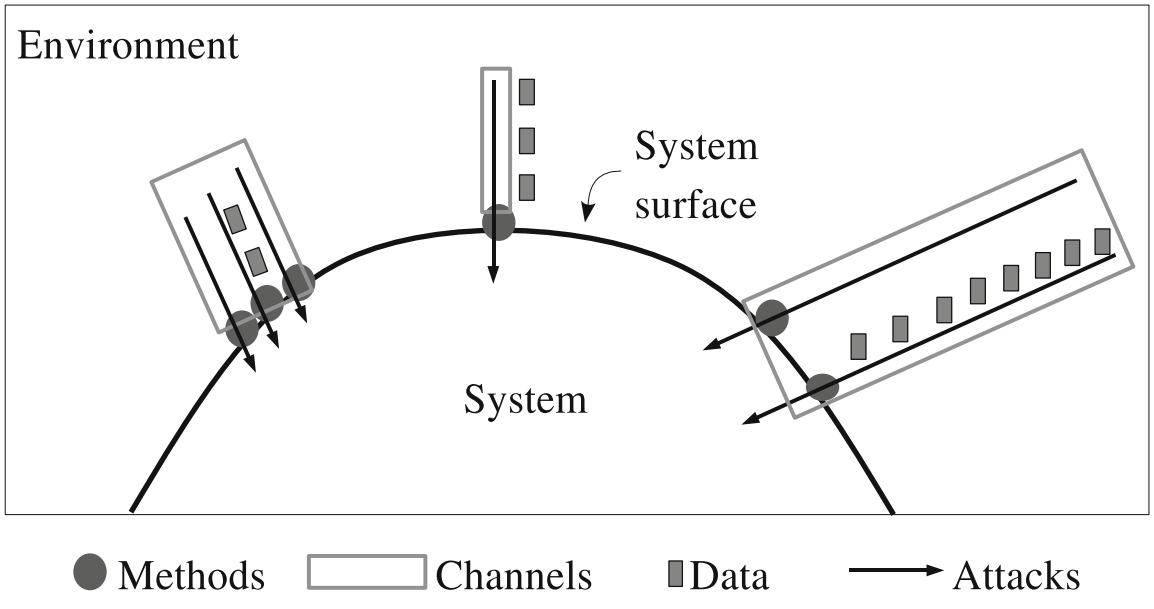
\includegraphics[width=0.7\linewidth]{img/system_attack_surface.png}
  \caption{System's Attack Surface\cite{mtd_vol1}}
  \label{fig:system_attack_surface}
\end{figure}

While the framework may be used in MTD, we can derive a better model for this usecase. New security models have been developed and measured \cite{mtd_security_model} \cite{mtd_book2} \cite{mtd_security_model_metric}. To have a better grasp of the problem encountered, an attack surface definition is in due. A system’s attack surface is the subset of the system’s resources that an attacker can use to attack the system. The taxonomy of the attack surface may be categorised into more smaller elements.

\subsubsection{Entry Points}
A system's entry points are methods, such as the system's API, that receive data items from the environment. For instance, a direct entry point, like a method receiving input from a user or reading a configuration file, can be invoked by a user or system in the environment, read from a persistent data item, or invoke another system's API. Indirect entry points receive data from direct entry points.

\subsubsection{Exit Points}
The system's exit points are methods, such as the one writing to a log file, that send data items to the environment. A direct exit point, like a method invoked by a user or system receiving data results, can write to a persistent data item or invoke another system's API with data items as input. An indirect exit point sends data to a direct exit point.

\subsubsection{Channels}
Systems have communication channels, like TCP/UDP sockets or RPC end points, which users or external systems use to interact. Attackers exploit these channels to connect to the system and invoke methods, adding another potential avenue for attacks.

\subsubsection{Untrusted Data Items}
An attacker utilizes persistent data items to either indirectly inject data into the system or receive data indirectly from it. Examples of persistent data items include files, cookies, database records, and registry entries. For instance, a system may read from a file after an attacker writes into it, or vice versa. Consequently, persistent data items serve as another vulnerability for potential attacks on a system.

\begin{figure}[htbp]
  \centering
  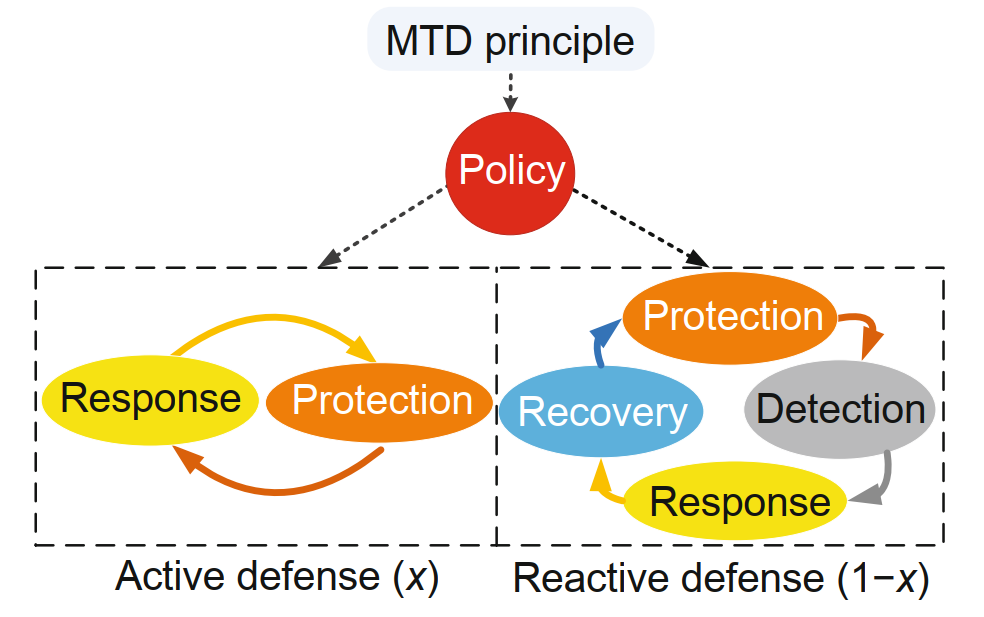
\includegraphics[width=0.7\linewidth]{img/mtd_new_ model.png}
  \caption{New Security Model for MTD\cite{mtd_security_model}}
  \label{fig:new_model}
\end{figure}


A new security model encompasses both active defense and reactive defense processes. In the active mode, defense operates independently of network status, periodically or irregularly shifting the attack surface. As a result, detection and recovery links are not required. In the reactive mode, the defense process is initiated by security alerts, aligning with the IPDRR model. x is the measurement of active defenses, and 1-x is the reactive defense measurement. A defense mechanism may employ a security system with different x, thus changing the dynamic.  
